\documentclass[a4paper,11pt,dvipsnames, twocolumn]{article}
\setlength{\columnseprule}{0.3pt}
\usepackage[a4paper,left=1.5cm,right=1.5cm,top=1cm,bottom=1.5cm]{geometry}
\usepackage{amsmath,amsthm,amssymb,amsfonts}
% \usepackage{array}
\usepackage{booktabs}
\usepackage[table]{xcolor}
\usepackage{cuted}
\usepackage{xcolor}
\usepackage{graphicx}
\graphicspath{{./img/}}
\usepackage{setspace}
\newcommand*\diff{\mathop{}\!\mathrm{d}}
\newcommand*\Diff[1]{\mathop{}\!\mathrm{d^#1}}
\usepackage{enumitem}

\usepackage[utf8]{inputenc}
\usepackage[T1]{fontenc}
\usepackage[spanish]{babel}


\usepackage{tabularx}
\newcolumntype{Y}{>{\centering\arraybackslash}X}




\usepackage[locale=FR, per-mode=fraction, separate-uncertainty=true]{siunitx}
\usepackage{physics}
\AtBeginDocument{\RenewCommandCopy\qty\SI}

\usepackage{pgfplots}
\usepackage{adjustbox, tikz}
\usepackage{tikz-3dplot}
\usepackage{circuitikz}
% \usepackage{gnuplottex}

% \usepackage{ifpdf}
\ifpdf%
  \usepackage{pdftricks}
  \begin{psinputs}
    \usepackage{pst-optic}
%\usepackage{pstricks-add} 	
  \end{psinputs}
\else
  \usepackage{pst-optic}
  \newenvironment{pdfpic}{}{}
\fi
 

\usetikzlibrary{decorations}
\usetikzlibrary{decorations.pathmorphing}
\usetikzlibrary{shapes.geometric}
\usetikzlibrary{arrows}
\usetikzlibrary{arrows.meta}   %edg
\usetikzlibrary{calc}
\pgfplotsset{compat=newest}
\usetikzlibrary{patterns}

\def\cosa{-0.69466}
\def\sina{-0.71934}
% A custom arrowhead for use on x, y, z axes
\tikzstyle{axisarrow} = [-{Latex[inset=0pt,length=5pt]}]


\usepackage{pgffor}
\usepackage{readarray}

% --------------------------------------
% Formatting the header.
\def\M{30} % Number of columns in header.
\def\N{27} % Columns for questions (can be different to actual number of questions).
\def\P{3} % Columns reserved for Total.

% Number of questions and points.
% --------------------------------------


% % --------------------------------------
% % Data for questions.
% % Don't remove the '%' after \data{
% \def\data{%
% A 5.0 26 520 9.77 80
% B 2.4 26 520 6.50 70
% C 5.0 32 592 5.55 30
% D 6.0 32 592 4.44 30
% }
% \readarray\data\dataA[4,6] %read the data to \dataA
% % --------------------------------------


\usepackage[most]{tcolorbox}
% A style for tcolorbox without frame etc. "notcb"
\tcbset{notcb/.style={enhanced jigsaw, colback=white, coltitle=black,sharp corners, boxrule=0pt}}
% Style for the number tables
\tcbset{tabularheader/.style={arc=2pt,notcb,boxsep=0pt,left=0pt,colbacktitle=white,rounded corners=all,enhanced jigsaw,coltitle=black,tabularx={*{8}{Y|}Y},boxrule=1pt,attach boxed title to top left, boxed title style={enhanced jigsaw,sharp corners,left=0pt,boxrule=0pt}}}

\begin{document}

\pagenumbering{gobble}

% \foreach \j in {1,...,4} {

% Nombres y Apellido: el Código Civil y Comercial estableció el uso de un solo
% apellido, de cualquiera de los padres, y de manera opcional el del otro progenitor


\begin{strip} %place some material in full-width at any place on double-column page
  \vspace{-1.25cm}
\begin{tcolorbox}[colback=white]

\begin{tcbraster}[raster columns=4,raster equal height]
  \begin{tcolorbox}[notcb,fontupper=\bfseries\raggedright]
    {\Large \vphantom{y}Física II}\par
    2$^\circ$ 31
  \end{tcolorbox}
  \begin{tcolorbox}[raster multicolumn=2, notcb,fontupper=\bfseries\centering]
    % \centering
    {\Large \vphantom{y} Recuperatorio del 2\textsuperscript{do} parcial}\par
    13 de diciembre de 2024
    % PARA REVISAR
  \end{tcolorbox}
  \begin{tcolorbox}[notcb,fontupper=\bfseries\raggedleft]
    \input{logoFRA_recortado}
    % 
\includegraphics[scale=0.2]{logoFRA_2022-recortado.png}
  \end{tcolorbox}
\end{tcbraster}
\begin{tcbraster}[raster columns=1, raster column skip=0pt, raster equal height,colback=white,before skip=0pt]
  \begin{tcolorbox}[coltitle=black,enhanced jigsaw,boxrule=0.5pt,boxsep=0pt,segmentation style={solid,black,line width=0.5pt},sidebyside,righthand width=9cm,fontupper=\tiny, fontlower=\tiny]
    Apellido
    \bigskip
    \tcblower
    Nombres
    \bigskip
  \end{tcolorbox}
\end{tcbraster}

\begin{tcbraster}[raster columns=\M, raster equal height,colback=white,before skip=0pt, boxsep=0.5pt]
  \begin{tcolorbox}[raster multicolumn=\N,tabularheader]
  % \begin{tcolorbox}[raster multicolumn=\N,tabularheader,title={\footnotesize some nice title}]
1 {\small ($2.5$ pts)}\par   \medskip\bigskip\bigskip & 2 {\small ($2.5$ pts)} & 3 {\small ($2.5$ pts)} & 4 {\small ($2.5$ pts)} & I & II & III
  %  1 (a) \par \bigskip\bigskip & 1 (b) \par  & 2 (a) \par  & 2 (b) \par  & 3 (a) \par  & 3 (b) \par & 4 \par 
  \end{tcolorbox}
  \begin{tcolorbox}[raster multicolumn=\P, colback=white,left=2pt,right=2pt]
    Nota

    \bigskip
    \bigskip
  \end{tcolorbox}
\end{tcbraster}

\end{tcolorbox}
% \textbf{Justificar todas las respuestas.} \hfill (\dataA[\j,1])
\textit{Para alcanzar la condición de Aprobación con Final debe sumar 4 puntos o más en los problemas 1 a 4. Para alcanzar la condición de Aprobación Directa debe sumar 6 puntos o más en los problemas 1 a 4, y responder correctamente al menos 2 de las preguntas I a III. \textbf{Justificar todas las respuestas.}}
\end{strip}


\begin{enumerate}[wide, labelwidth=2pt, labelindent=0pt]
  % [leftmargin=*]


\item La figura muestra una espira cuadrada de lado $b=3,0\text{ cm}$, en el mismo plano que contiene un cable muy largo, y a una distancia $a=2,0\text{ cm}$ de dicho cable. Por el cable circula una corriente $i_1=5,0\text{ A}$ y por la espira una corriente $i_2=2,5\text{ A}$. Hallar el vector de la fuerza ejercida sobre el segmento $AB$ debida a la presencia del campo magnético generado por la corriente $i_1$.
\begin{center}
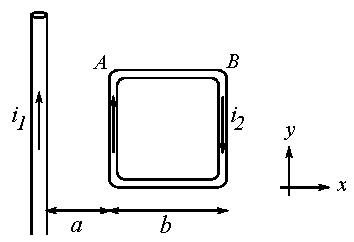
\includegraphics[scale=1]{2019_p3_fuerza_segmento.pdf}
\end{center}

\item En el circuito de la figura, los valores de las resistencias y las baterías son:\\
$R_1 = 5,0\text{ k}\Omega$; $R_2 = 3,0\text{ k}\Omega$; $R_3 = 1,0\text{ k}\Omega$; $R_4 = 1,5\text{ k}\Omega$; $\varepsilon_1 = 12\text{ V}$; $\varepsilon_2 = 24\text{ V}$.\\
a) Calcule la potencia entregada por la batería $\varepsilon_2$.\\
b) Calcule el potencial en el punto $a$.
\begin{center}
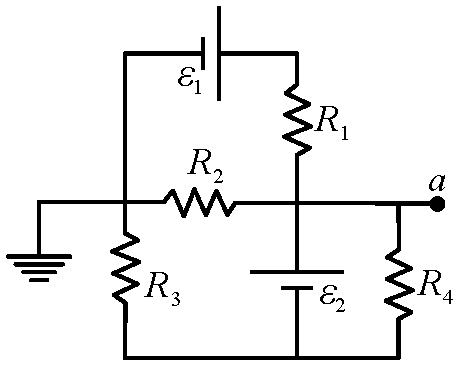
\includegraphics[scale=0.8]{2019_p2_circuito.pdf}
\end{center}

\item Una espira cuadrada cuyos lados miden $0.25\,\text{m}$ se mueve con velocidad constante $\vec{v}=30\text{ m/s }\hat{x}$, como se muestra en la figura. La espira se encuentra en una región donde está presente el siguiente campo magnético:
\begin{flalign*}
\vec{B} &= B_0 (1+ax)\hat{z}\,,
\end{flalign*}
donde $B_0=0.7\text{ T}$ y $a=2.0\text{ m}^{-1}$. La resistencia eléctrica de la espira es $2\text{ }\Omega$.\\
a) Calcule la f.e.m. inducida en la espira.\\
b) Calcule la fuerza externa que debe ser aplicada sobre la espira para que su velocidad se mantenga constante.
\begin{center}
\hspace{5pt}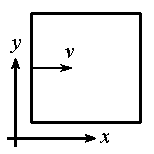
\includegraphics[scale=1]{2019_p3_rec_espira.pdf}
\end{center}

\item En el circuito de la figura, los dos capacitores están inicialmente cargados y en equilibrio, con la llave abierta. La capacidad del capacitor 1 es $C_1 = \SI{20}{\micro\farad}$ y la capacidad del capacitor 2 es desconocida. La llave se cierra en el instante $t_0 = 0$, y en el instante $t_1 = \SI{595}{\micro\second}$ se mide que la corriente es el $22.6\%$ de la corriente máxima observada en este circuito. Calcular la capacidad $C_2$.
%
\begin{center}
\begin{circuitikz}[scale=0.8]
\draw (0,0) to[C, l=$C_1$] (0,1.5) to[C, l=$C_2$] (0,3) to[switch] (4,3) to[R=$\SI{50}{\ohm}$] (4,0) to[R=$\SI{30}{\ohm}$] (0,0);
\end{circuitikz}
\end{center}

\end{enumerate}


\vspace*{\fill}

\begin{flushright}
\textbf{Sigue atrás.}
\end{flushright}
\newpage

\begin{enumerate}[label=\roman*., wide, labelwidth=!, labelindent=0pt]

\item ¿Cómo puede determinarse la dirección de un campo magnético únicamente con observaciones cualitativas de la fuerza magnética sobre un alambre recto que transporta corriente?
\item Un rectángulo de metal está cerca de un alambre largo, recto y que conduce corriente, como muestra la figura. Si la corriente en el alambre está disminuyendo, ¿el rectángulo es repelido o atraído por el alambre? 
\begin{center}
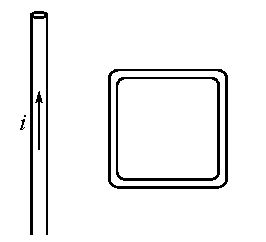
\includegraphics[scale=0.9]{2019_p3_feb3_rectangulo_y_cable.pdf}
\end{center}

\item Explique si la potencia entregada por la batería aumenta, disminuye o no cambia, cuando al circuito mostrado en la figura se conecta un voltímetro real (no ideal) en los puntos indicados.
\begin{center}
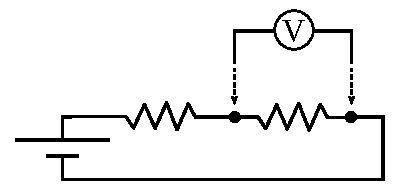
\includegraphics[scale=1]{2018_p3_FEB2_II.pdf}
\end{center}

\end{enumerate}


\end{document}
